\section{Introduction}\label{intro}\sloppy
The availability of data and vast cloud-based computational resources is continues the path towards the use of more sophisticated machine learning (ML) models in data science applications for prediction, recommendation and automation.
The database community has built systems that support almost every stage of the development process including featurization~\cite{keystone,zhang2014mat}, distributed model training~\cite{hellerstein2012madlib, crotty2014tupleware, feng2012towards, tensor}, and model deployment~\cite{crankshawmissing}.  
However, an under-served, yet crucial, component of the data science process is the management and cleaning of dirty data.  Such data errors can occur in the data used for training the ML models as well as the data that the models make predictions for.  This dirty data, if unaccounted for, can drastically bias the model's predictions and lead to incorrect predictions that are undesirable or even dangerous~\cite{vanderbilt2012let}.  Recent papers and surveys of analysts suggest that such effects due to dirty data are pervasive in data science and predictive applications~\cite{sculley2014machine,kandel2012,krishnan2016hilda}.

% In the context of ML, dirty data refers to unintended or unpredictable numerical features that arise from a violation of an invariant expected by the developer (e.g., un-handled NULL values being automatically mapped to 0).  Dirty data affects both the model training and any future predictions the application might make, and numerous papers~\cite{sculley2014machine} and surveys of analysts~\cite{kandel2012, krishnan2016hilda} suggest that the effects and costs of dirty data are pervasive.

%that it takes significant effort to manually identify dirty data and design software to mitigate their effects 

\iffalse
\begin{figure}[t]
% \vspace{-5pt}
\centering
 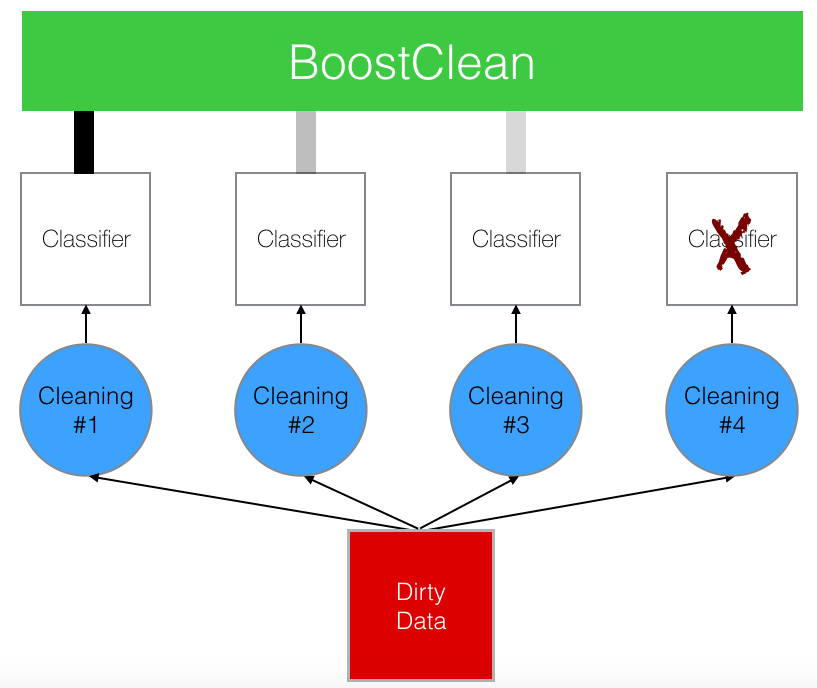
\includegraphics[width=0.8\columnwidth]{figures/teaser.png}
 \caption{ \sys is a new data cleaning system that detects errors in ML data and adaptively selects from a set of repair actions to maximize prediction accuracy. This selection problem is formulated as a statistical boosting procedure, which reweights the data to focus on model mispredictions.
 \label{fig:teaser}}
\end{figure}
\fi

As a concrete example, we are collaborating with a data science company called \company\footnote{Anonymized at the request of the company.} that ranks sales leads. The company aggregates clients' Salesforce.com data on past sales leads, integrates this data with additional information scraped from the web about the client and those leads, and trains a classification model that predicts the success of future uncontacted leads.  Because the data are acquired from a combination of manual data entry and automatically scraped web data, inconsistencies, missing data, and incorrect values are a significant problem.  For instance, a typical error is the inconsistent representation of missing values (e.g., ``-999'', ``EMPTY'' or ``none'' may be used depending on the sales representative).  If the featurization code does not recognize and address these errors, it can lead to biases that degrade the quality of the model. For example, the data scientist may impute a default mean value for all blank attributes but miss the code ``-999'', which is then interpreted as a semantic value. 
At the company, detecting and repairing errors takes roughly 1 week of human manual work per dataset. 
Furthermore, the company has heterogeneous data and this effort will have to be spent each time a new dataset is used.

Surveys suggest that this company's data cleaning challenges are not unique and are prevalent in many industrial ML pipelines~\cite{krishnan2016hilda}.  
Software Engineers write custom conditional cleaning scripts that are a combination of a {\it detector}, which are a collection of Boolean functions that specify a subset of records that are dirty, and {\it repair} functions that transform or delete those records.  It is not enough to write these scripts once, as the predictive nature of ML applications means that they are continuously encountering new, unseen data.
Software Engineers must constantly monitor and maintain the data processing pipeline to account for unexpected changes to the input data~\cite{sculley2014machine, DBLP:conf/sigmod/KrishnanFGWW16}.
To further exacerbate this problem, modern prediction models rely on data integrated from a wide variety of sources (e.g., \company combines on average 5-10 sources to train a model).  For each data source, the Engineer must understand domain-specific information (e.g., invariants) in order to accurately clean the data.

To reduce this burden, we present a new system, called \sys, that automates the process of detecting and repairing a common class of data errors called {\it domain value violations} that occur when an attribute value is outside of its value domain.  Although seemingly simple, numerous data quality surveys across the database, statistics, and scientific literature~\cite{muller2005problems,li2010improving,kim2003taxonomy,kandel2011research} highlight the prevalence, variety, and importance of this class of errors, which can manifest in the form of missing data, incorrect data, or inconsistent representations of the same logical data value.  By focusing on this common but simpler class of errors, Software Engineers can focus resources on more complex scenarios such as entity resolution.   In addition, by automating this aspect of data cleaning, \sys can help ensure that deployed models maintain high accuracy even in the presence of dirty data, and engineers are only needed to address drastic changes to the input data. 

Data cleaning for such data science applications presents novel characteristics not present in traditional data cleaning settings that we can exploit in \sys.  First, our goal is not to fully clean each record; instead, we leverage our access to the downstream predictive model to tailor the cleaning operations towards improving the model accuracy.  Recent work finds tha customizing data cleaning to downstream applications can significantly reduce cleaning costs~\cite{altwaijry2015query, DBLP:conf/sigmod/BergmanMNT15, DBLP:journals/pvldb/KrishnanWWFG16}.
Second, test data is often available (e.g., the results of following a sales lead) and can be used to evaluate the results of data cleaning.  In \sys, our only assumption is that the test labels (e.g., whether a customer purchased an item) are correct; the attribute values are allowed to contain errors.  In contrast, traditional data cleaning relies on access to a clean dataset where {\it all attributes are fully correct}.  We leverage the test data to evaluate the impact of a given cleaning operation on whether it will improve or hurt a model's prediction accuracy.  The key challenge is to efficiently search the space of possible conditional data cleaning scripts (detector and repair combinations), while ensuring that the model does not overfit~\cite{DBLP:journals/pvldb/KrishnanWWFG16,krishnan2016hilda}.   

Our primary observation is that a given conditional cleaning script can be interpreted as generating a new set of features (the cleaned values), ad thereby generate a new model trained on those cleaned features. 
We can view the process of selecting the best sequence of cleaning operations as an ensembling problem, i.e., selecting the best collection models that collectively estimate a label. 
Although there are many possible algorithms~\cite{dietterich2000ensemble}, we use a powerful technique called Boosting~\cite{freund1995desicion} that composes a set of weak learners into a strong learner.  
First, unlike methods that are specific to certain classes of models (e.g., linear models, differentiable models), boosting can be applied to black-box models. 
Second, it takes interactions and correlations between the different data cleaning models into account by incrementally selecting ``orthogonal'' compositions.


% is similar cleaning operations can be viewed as collections of feature extraction operations, and consequently, automated feature selection techniques can be adopted to the data cleaning setting.  For example, consider a cleaning operation that fills an empty attribute value with a default value.  The default value may be the most common value in the dataset, the mean value, or even a random attribute value in the dataset; every default value setting corresponds to a specific {\it instance} of a cleaning operation, and can be viewed as a separate feature extraction function.  Thus the goal is to select a sequence of cleaning operation instances that maximizes the downstream model's test accuracy.


\sys takes as input a relational table, a library of detector functions $\mathcal{D}$ that generate (possibly incorrect) predicates that match candidate dirty records, a library of repair functions $\mathcal{F}$ that transform or delete a record, and a user-specified classifier training procedure \texttt{train()}.
\sys has two key components: an automatic error detector to determine subsets of records that are dirty, and a repair selector to select repair actions for those dirty records using boosting.
We cast the former component into a featurization problem, so that the user focuses on the familiar task of creating feature extraction functions while \sys translates these features into error detection rules using a technique called Isolation Forests~\cite{liu2008isolation}.  Further, we have written a general set of featurizers, including one that is a novel adaptation of the \textsf{word2vec} neural network architecture that is effective at detecting multi-attribute errors.  The neural network can be individually tailored to each dataset and learn to predict the co-occurrence of attributes in a record. 
The detectors output relational predicates $p_i$, which can be used to detect candidate errors.  The second component then uses boosting to generate a sequence of conditional cleaning scripts $(p_i, r_i)$ to be applied to the training and test datasets, where $r_i$ is the repair function to be applied on records matching predicate $p_i$.

This paper focuses on data errors that cause domain value violations in the context of supervised classification models (both single and multi-class).  The system is currently designed for a single-node setting. Our contributions are as follows:

\vspace{0.25em}\noindent\textbf{Boosting: } We present a new automated data cleaning system based on statistical boosting that finds the best ensemble of operations from a library of operations to maximize the predictive performance of a downstream model. We evaluated \sys on a collection of datasets from machine learning competitions, real-world data analyses, and \company, and improved prediction accuracy by up to $14.5\%$ in comparison to baseline approaches on completely unseen test data. 

\vspace{0.5em}\noindent\textbf{Error Detection Library: } We have built an optimized library of data cleaning operations based on deterministic rules and statistical criteria from which \sys selects. To better detect errors in categorical attributes, we developed a novel detector based on the \textsf{Word2Vec} neural network architecture. Following prior experimental procedures~\cite{DBLP:journals/pvldb/AbedjanCDFIOPST16}, the library achieves a detection accuracy of 81\% of all of the errors found by hand-written rules on 8 machine learning datasets.  %\sys is on average 40\% more accurate than applying statistical outlier detection to only the quantitative attributes.

\vspace{0.5em}\noindent\textbf{Optimizations: } Our parallelization of the boosting procedure results in a $9.7\times$ on a $16$-core machine, while our indexing and materialization optimizations achieve an additional $10\times$ for a 1.5GB dataset.

% and indexing-based optimizations speed up the boosting and repair selection  We demonstrate how we can parallelize the inner-loop of the boosting operation, and on a 16-core machine \sys achieves a 9.7x speedup for the repair selection step. Similarly, we show that building an index can speed up operator selection .






\iffalse
The problem of dirty training data in ML is subtle as most learning algorithms are robust to statistical noise.
However, un-modeled systematic biases in the training data can still adversely affect the results~\cite{DBLP:journals/pvldb/KrishnanWWFG16, DBLP:conf/case/MahlerKLSMKPWFAG14, xiaofeature}.
The way that the developer chooses to address corruption will have a significant impact on the performance of the ML application.
Consider a music recommender system where a recent software update causes songs longer than 5 minutes to have ``NULL'' ratings.
If the ML developer treats a NULL rating as ``0 stars'', those songs may never get recommended.
To avoid this bias, it may be more prudent to discard those ratings or impute a default  value (e.g., mean over all previous non-NULL ratings).

To setup the abstract search problem, we are given a dataset $R$, a library of data cleaning operations $\mathcal{L}=\{l_1,...,l_k\}$, a user-specified model training program which returns a classifier, and an oracle that evaluates the prediction accuracy of the classifier (e.g., a ground truth clean test dataset).
Our objective is to find a classifier that maximizes prediction accuracy by applying compositions of operators in our library to $R$ and training on the resulting dataset.
While this problem is inherently combinatorial, the key insight is to model the hypothesis testing procedure as a form of adaptive statistical boosting. 
\fi




%The datasets are inconsistent in the way they represent missing information (e.g., some numerical fields left blank, some fields with a placeholder value of ``-999''). 
%Featurization code that does not recognize that a blank attribute value is semantically equivalent to a ``-999'' attribute value can lead to biases--for example, the data scientist may impute a sensible default mean value for all of the blank attributes but treat the ``-999'' as the given value.

\if{0}
Clearly, some level of automation in detecting and handling erroneous data can reduce the burden on data scientists.
Automated rule-based data repair is a well-studied field~\cite{DBLP:conf/sigmod/ChuIKW16}, but the ML setting presents additional challenges and structure that are important to understand.
In ML, incoming records are, in a sense, both data (during training) and queries (during prediction).
This provides additional degrees-of-freedom in handling dirty data.
For example, when asked to predict a label for a dirty example, one may want to return a ``fail-safe'' prediction instead of cleaning it first and then asking for a prediction.
Second, ML applications often have a way of measuring prediction accuracy.
Labels often represent directly observed user-behavior (e.g., sale vs. no sale, whether the user clicked a link etc.), and thus, are relatively consistent over the lifetime of an application.
On the other hand, the features used to predict the labels may be integrated from a variety of different company databases and susceptible to inconsistencies and change.
With this in mind, we present \sys, a new data cleaning system that detects errors in ML data and uses knowledge of the labels to adaptively select from a set of repair actions to maximize prediction accuracy.
\fi